% 	Name		:: 	sthlm Beamer Theme  HEAVILY based on the hsrmbeamer theme (Benjamin Weiss)
%	Author		:: 	Mark Hendry Olson (mark@hendryolson.com)
%	Created		::	2013-07-31
%	Updated		::	June 18, 2015 at 08:45
%	Version		:: 	1.0.2
%	Email		:: 	hendryolson@gmail.com
%	Website		:: 	http://v42.com
%
% 	License		:: 	This file may be distributed and/or modified under the
%                  	GNU Public License.
%
%	Description	::	This presentation is a demonstration of the sthlm beamer
%					theme, which is HEAVILY based on the HSRM beamer theme created by Benjamin Weiss
%					(benjamin.weiss@student.hs-rm.de), which can be found on GitHub
%					<https://github.com/hsrmbeamertheme/hsrmbeamertheme>.


%-=-=-=-=-=-=-=-=-=-=-=-=-=-=-=-=-=-=-=-=-=-=-=-=
%
%        LOADING DOCUMENT
%
%-=-=-=-=-=-=-=-=-=-=-=-=-=-=-=-=-=-=-=-=-=-=-=-=

\documentclass[newPxFont]{beamer}
\usetheme{sthlm}
%\usecolortheme{sthlmv42}

%-=-=-=-=-=-=-=-=-=-=-=-=-=-=-=-=-=-=-=-=-=-=-=-=
%        LOADING PACKAGES
%-=-=-=-=-=-=-=-=-=-=-=-=-=-=-=-=-=-=-=-=-=-=-=-=
\usepackage[utf8]{inputenc}
\usepackage[T1]{fontenc}

%\usepackage{chronology}
\usepackage{chronosys}
\usepackage{subfigure}
\usepackage{multimedia} %Embedding videos and animations
%\usepackage{movie9}

\newcommand{\tabitem}{%
  \usebeamertemplate{itemize item}\hspace*{\labelsep}}

%\renewcommand{\event}[3][e]{%
%  \pgfmathsetlength\xstop{(#2-\theyearstart)*\unit}%
%  \ifx #1e%
%    \draw[fill=black,draw=none,opacity=0.5]%
%      (\xstop, 0) circle (.2\unit)%
%      node[opacity=1,rotate=45,right=.2\unit] {#3};%
%  \else%
%    \pgfmathsetlength\xstart{(#1-\theyearstart)*\unit}%
%    \draw[fill=black,draw=none,opacity=0.5,rounded corners=.1\unit]%
%      (\xstart,-.1\unit) rectangle%
%      node[opacity=1,rotate=45,right=.2\unit] {#3} (\xstop,.1\unit);%
%  \fi}%

%-=-=-=-=-=-=-=-=-=-=-=-=-=-=-=-=-=-=-=-=-=-=-=-=
%        BEAMER OPTIONS
%-=-=-=-=-=-=-=-=-=-=-=-=-=-=-=-=-=-=-=-=-=-=-=-=

%\setbeameroption{show notes}

%-=-=-=-=-=-=-=-=-=-=-=-=-=-=-=-=-=-=-=-=-=-=-=-=
%
%	PRESENTATION INFORMATION
%
%-=-=-=-=-=-=-=-=-=-=-=-=-=-=-=-=-=-=-=-=-=-=-=-=

\title{Perceptions de l’arbre en contexte sahelien}
\subtitle{Proposition de l’OHMi Tessekere \\
 ANR « FUTURE SAHEL »}
%\date{\small{\jobname}}
%\date{\today}
\date{8-12 mai 2017}
\author{\texttt{ K. Niang, E. Delay, J.-L. Peiry, D. Goffner}}
\institute{\textsc{Ohm} Téssékéré - Sénégal}

\hypersetup{
pdfauthor = {E. DELAY},
pdfsubject = {Ateliers du réseau OHM},
pdfkeywords = {grande muraille verte, ANR future Sahel},
pdfmoddate= {D:\pdfdate},
pdfcreator = {}
}

\begin{document}

%-=-=-=-=-=-=-=-=-=-=-=-=-=-=-=-=-=-=-=-=-=-=-=-=
%
%	TITLE PAGE
%
%-=-=-=-=-=-=-=-=-=-=-=-=-=-=-=-=-=-=-=-=-=-=-=-=

\maketitle

%\begin{frame}[plain]
%	\titlepage
%\end{frame}

%-=-=-=-=-=-=-=-=-=-=-=-=-=-=-=-=-=-=-=-=-=-=-=-=
%
%	TABLE OF CONTENTS: OVERVIEW
%
%-=-=-=-=-=-=-=-=-=-=-=-=-=-=-=-=-=-=-=-=-=-=-=-=
%\section*{Overview}
%\begin{frame}{Overview}
%% For longer presentations use hideallsubsections option
%\tableofcontents[hideallsubsections]
%\end{frame}

%-=-=-=-=-=-=-=-=-=-=-=-=-=-=-=-=-=-=-=-=-=-=-=-=
%	FRAME: INTRODUCTION
%-=-=-=-=-=-=-=-=-=-=-=-=-=-=-=-=-=-=-=-=-=-=-=-=

\section{Introduction}

%-=-=-=-=-=-=-=-=-=-=-=-=-=-=-=-=-=-=-=-=-=-=-=-=
%	FRAME: CONTEXT
%-=-=-=-=-=-=-=-=-=-=-=-=-=-=-=-=-=-=-=-=-=-=-=-=
\begin{frame}[c]{Context de l'étude}
\vspace{-1cm}
% Questionnement autour de la place de l'arbre
\begin{itemize}
  \item Constat : des populations qui sont essentiellement centrées sur le pastoralisme.
  \item Objectif : comprendre la place "traditionnelle" des produits (services éco-systémiques) issus de l'arbre pour accroître la résilience socio-environnementale (e.g. diversification) des populations aux chocs : sécheresse, épidémie
\end{itemize}

Quels sont les usages des arbres en tant que pourvoyeur de ressources et vecteurs de services écosystémiques (médicinaux, cosmétiques, alimentaires, fourragers, etc.) ?

%Mieux comprendre sa dans l’espace perçu / vécu des populations pour favorier la gestion des ressources naturelles (stratégies de reboisement).
\begin{figure}
	\centering
	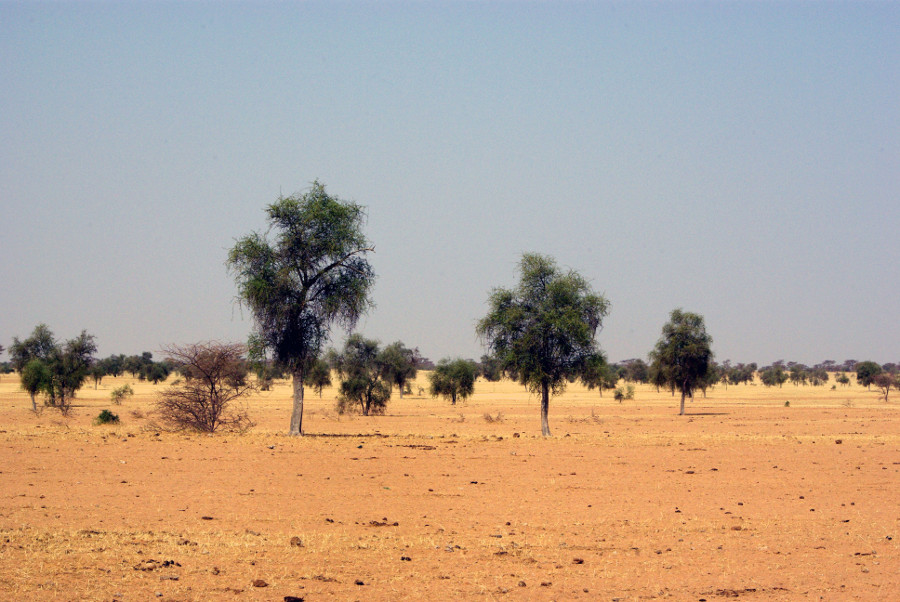
\includegraphics[width = 0.5\textwidth]{img/2007_Podor.JPG}
	\caption{FutureSahel Work Packages}
\end{figure}
\end{frame}

%-=-=-=-=-=-=-=-=-=-=-=-=-=-=-=-=-=-=-=-=-=-=-=-=
%	FRAME: Résilience et stockolm
%-=-=-=-=-=-=-=-=-=-=-=-=-=-=-=-=-=-=-=-=-=-=-=-=
\begin{frame}[c]{La résilience socio-environnementale : approche pratique}
\vspace{-1cm}
Peut-on considérer les services éco-systémiques rendus par l'arbre en contexte sahélien comme
facteur de résilience pour les populations et l'environnement?

L'OHM Téssékéré et l'ANR "future Sahel" travaillent avec le \textit{Stockholm Resilience Centre} sur l'application des concepts de résilience socio-environnementale à la zone de la grande muraille.

\begin{figure}
	\centering
	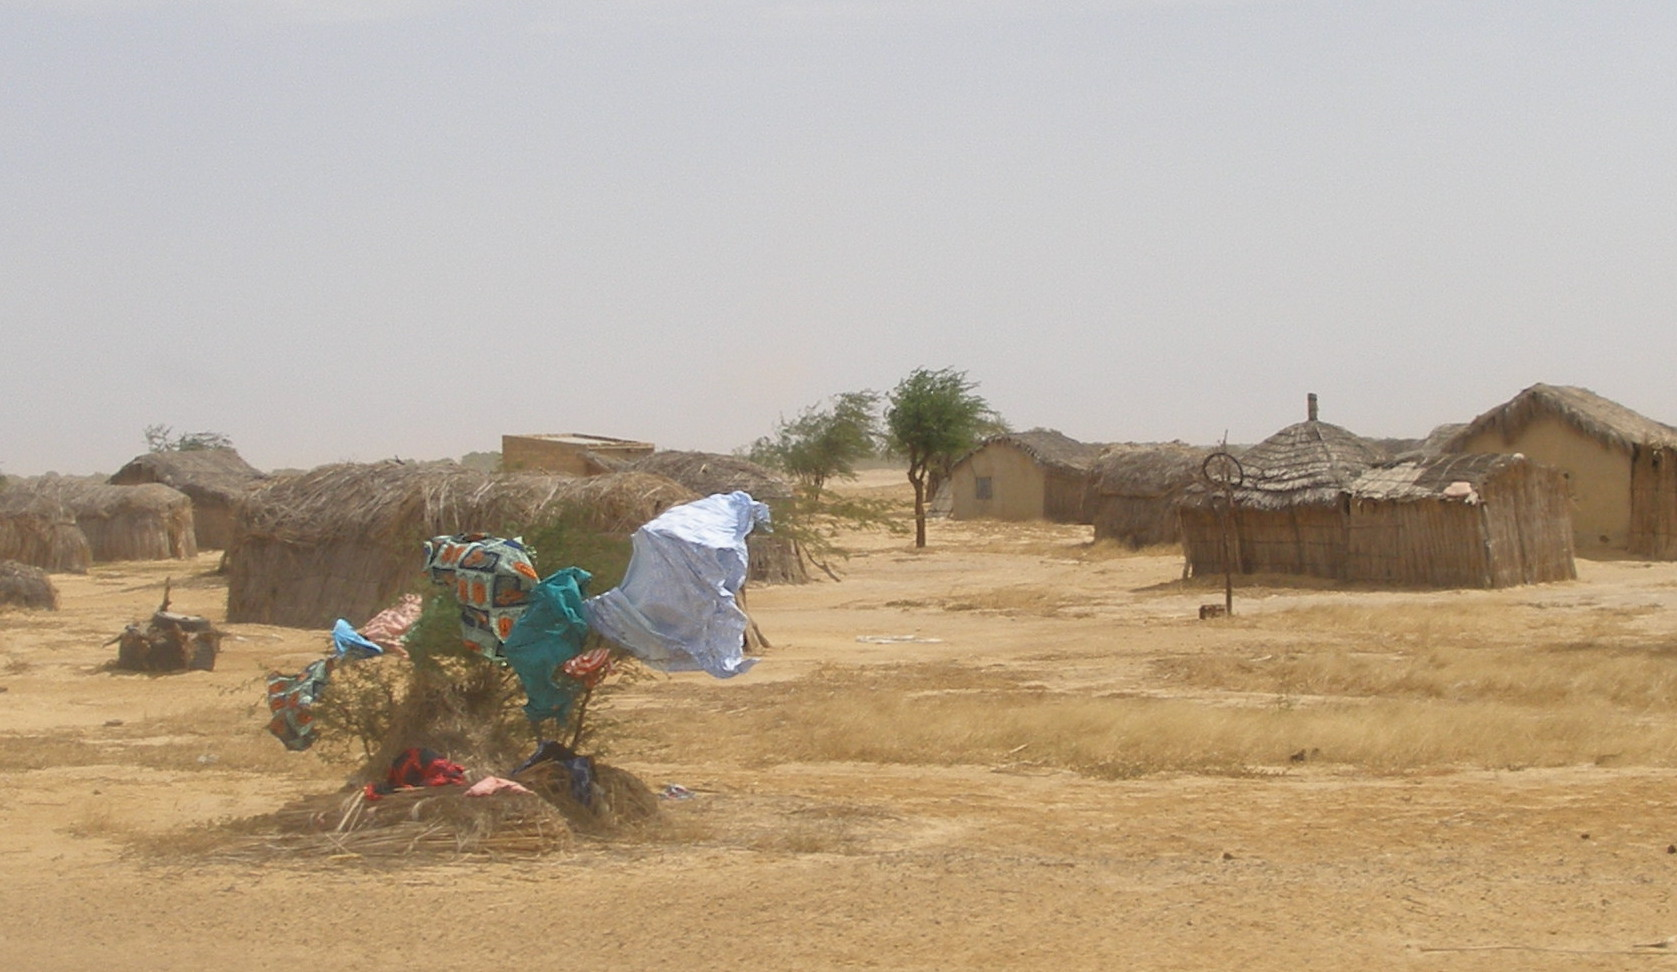
\includegraphics[width = 0.65\textwidth]{img/PA310152.JPG}
	\caption{FutureSahel Work Packages}
\end{figure}
\end{frame}


%-=-=-=-=-=-=-=-=-=-=-=-=-=-=-=-=-=-=-=-=-=-=-=-=
%	FRAME: Prospective
%-=-=-=-=-=-=-=-=-=-=-=-=-=-=-=-=-=-=-=-=-=-=-=-=
\begin{frame}[c]{Resilience et prospective}
\vspace{-1cm}

« Considérer l’avenir non comme une chose déjà décidée et qui petit à petit se
découvrirait à nous, mais comme une chose à faire dont la nature dépendra
à la fois de nos forces, de notre habileté, de notre courage, et d’un certain
nombre de circonstances que nous ne pourrons jamais prévoir dans tous leurs
détails.» (Berger 1967, p.33).

\begin{figure}
	\centering
	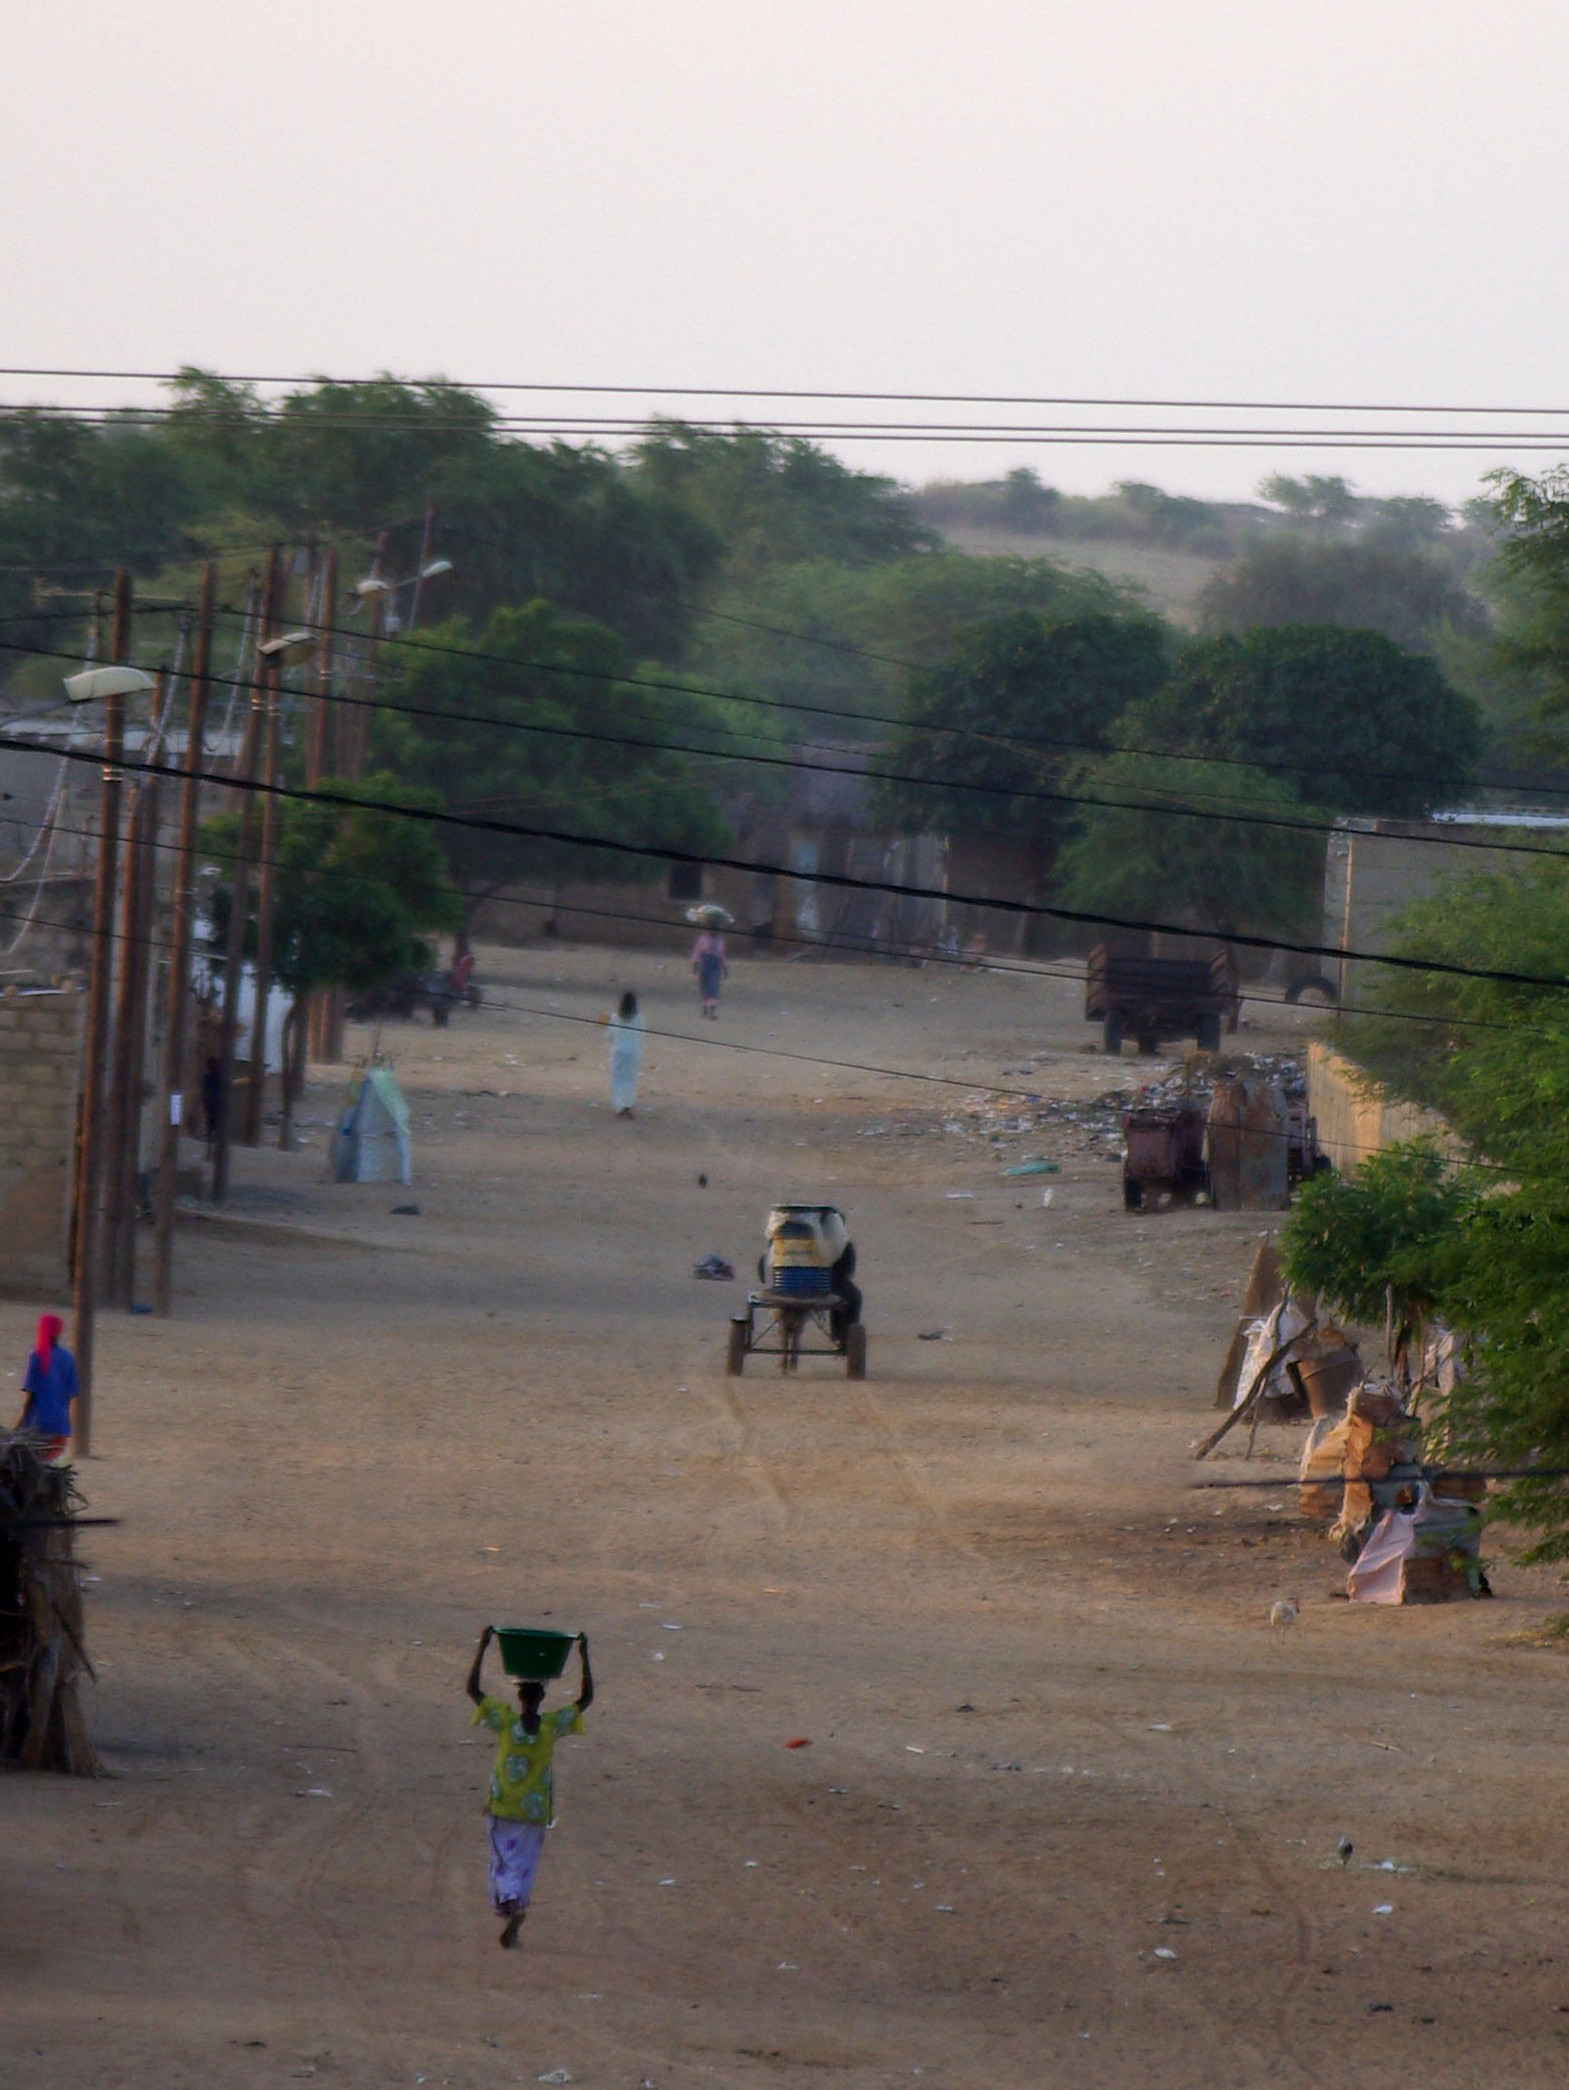
\includegraphics[width = 0.3\textwidth]{img/RossBethio_3424.JPG}
	\caption{FutureSahel Work Packages}
\end{figure}
\end{frame}

%-=-=-=-=-=-=-=-=-=-=-=-=-=-=-=-=-=-=-=-=-=-=-=-=
%	FRAME: Les fenetres GMV
%-=-=-=-=-=-=-=-=-=-=-=-=-=-=-=-=-=-=-=-=-=-=-=-=
\begin{frame}[c]{La grande muraille verte}
\vspace{-1cm}
Un travail réalisé sur des fenêtres avec une diversité de situations socio-spatiales.
\small{
\begin{itemize}
  \item Sakal : agro-pastoral (agriculture pluviale - arachide, mil, niébés, pastèque)
  \item Koeili-Alpha, Labgar : pastoral (brousse arborée essentiellement composée de \textit{Balanites} (dattier du désert))
  \item Ranerou : complexité des socio-éco patches (plus grande mixité).
\end{itemize}}
%Image googleEarth des fenetres
\begin{figure}
	\centering
	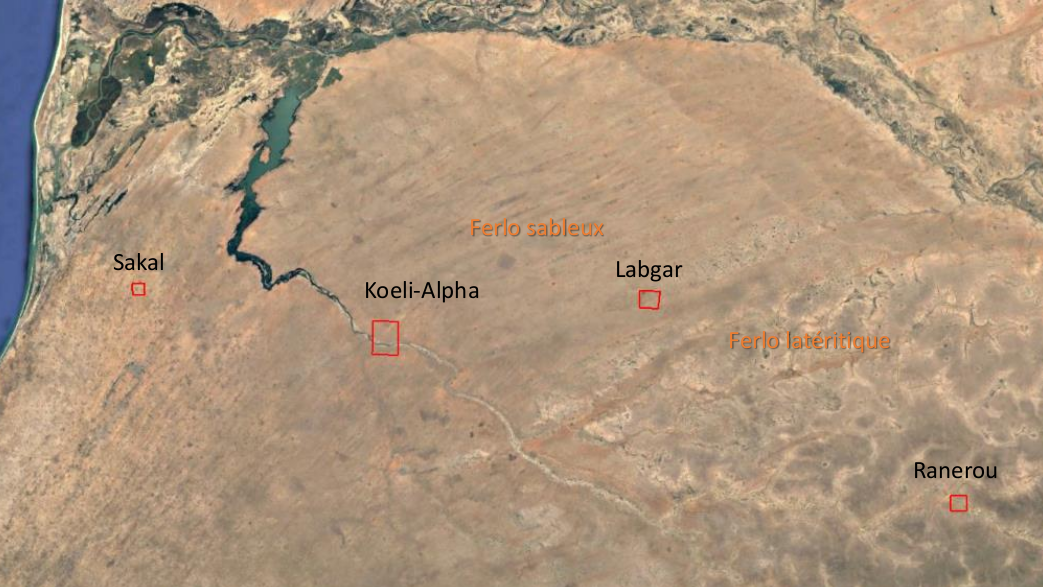
\includegraphics[width = 0.6\textwidth]{img/windows.png}
\end{figure}
\end{frame}

\section{methodologie - l'entree ethno-botanique}

%-=-=-=-=-=-=-=-=-=-=-=-=-=-=-=-=-=-=-=-=-=-=-=-=
%	FRAME: ethnobotanique
%-=-=-=-=-=-=-=-=-=-=-=-=-=-=-=-=-=-=-=-=-=-=-=-=
\begin{frame}[c]{Les entretiens ethnobotaniques}
\vspace{-1cm}

Entretiens semi-directifs structurés avec les acteurs (individuels et \textit{focus groups}) afin de comprendre la problématique et les réalités du terrain, de cerner les éléments essentiels à prendre en compte.

Connaître les usages, les stratégies de collecte, la saisonnalité, les modes de valorisation.

%Les entretiens se font en wolof et/ou poulard et son mener par plusieurs personnes en simultané sur les campements. Un brefing est réaliser au préalable pour explicier le guide d'entretien.

%acteurs photos jean-luc
\begin{figure}
	\centering
	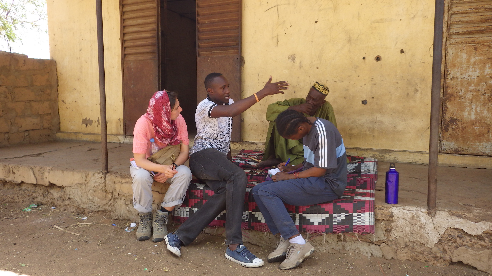
\includegraphics[height = 3.5cm]{img/group3.png}~
  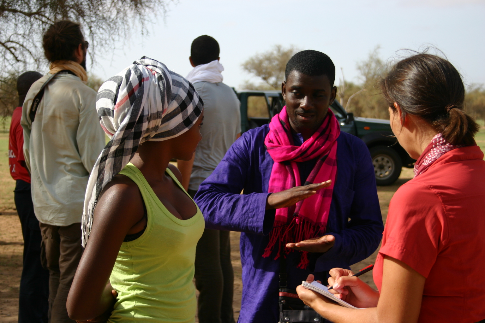
\includegraphics[height = 3.5cm]{img/group2.png}
\end{figure}
\end{frame}

%-=-=-=-=-=-=-=-=-=-=-=-=-=-=-=-=-=-=-=-=-=-=-=-=
%	FRAME: Questionnaires
%-=-=-=-=-=-=-=-=-=-=-=-=-=-=-=-=-=-=-=-=-=-=-=-=
\begin{frame}[c]{L'approche par questionnaires}
\vspace{-1cm}
Un questionnaire spécifique est utilisé pour quantifier les informations déjà obtenues dans les entretiens.

Réalisation de 30-40 questionnaires par sites (un total de 200 questionnaires pour l’ensemble des sites).
%Image googleEarth des fenetres
\begin{figure}
	\centering
	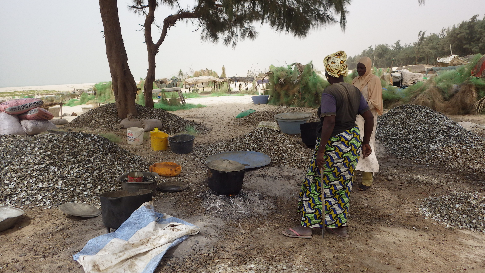
\includegraphics[width = 0.6\textwidth]{img/Khoudia.png}
\end{figure}

\end{frame}

%-=-=-=-=-=-=-=-=-=-=-=-=-=-=-=-=-=-=-=-=-=-=-=-=
%	FRAME: Ecologie du paysage
%-=-=-=-=-=-=-=-=-=-=-=-=-=-=-=-=-=-=-=-=-=-=-=-=
\section{methodologie - apports de l'ecologie du paysage}

\begin{frame}[c]{L'approche écologie du paysage 1/4}
\vspace{-1cm}
Un travail inspiré de la méthodologie proposé par Sinare \textit{et al.} (2016)
\begin{figure}
	\centering
	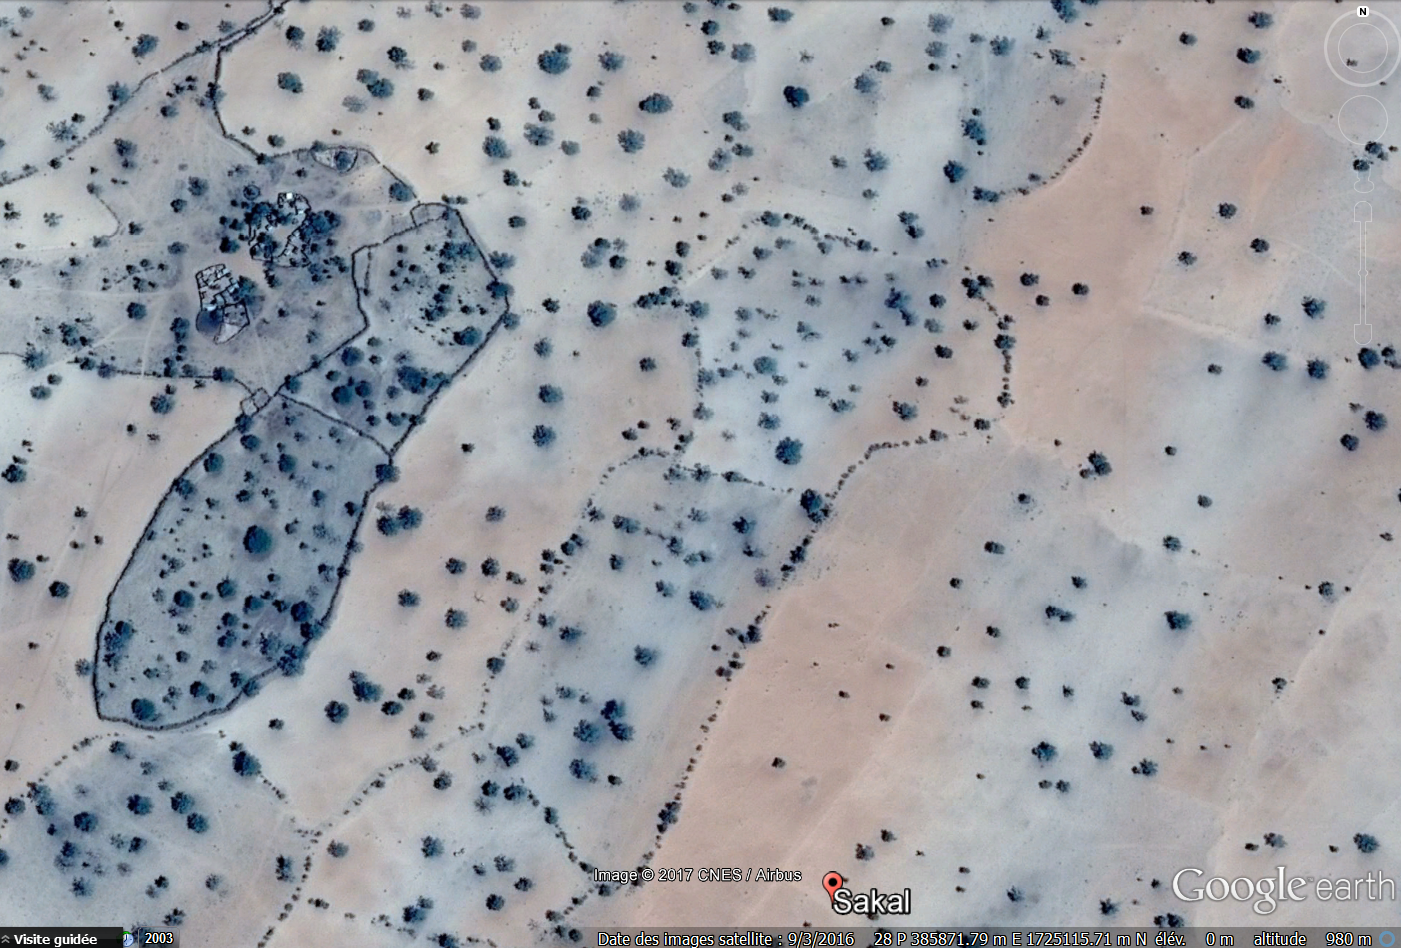
\includegraphics[height = 3.5cm]{img/ggearth}
  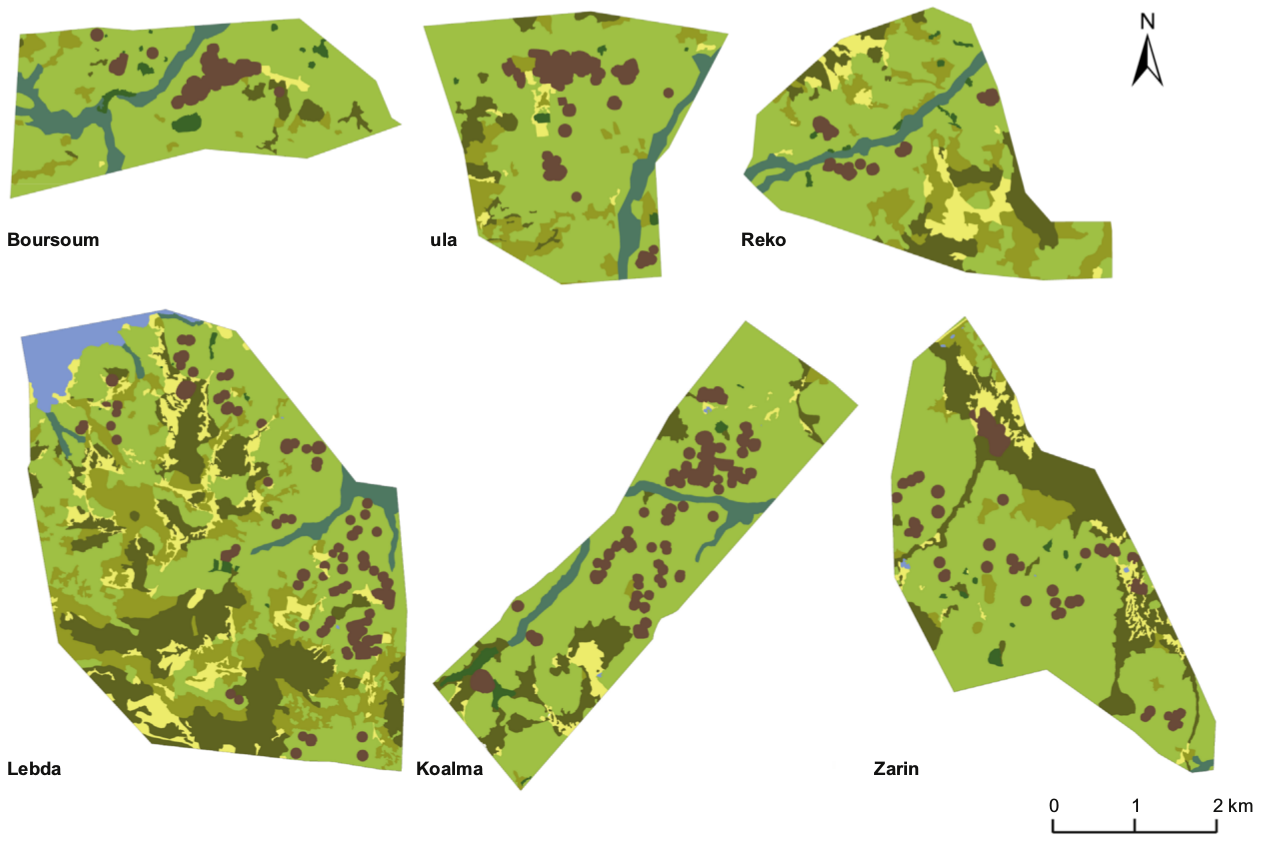
\includegraphics[height = 3.5cm]{img/Sinare_et_al2016}
  \caption{\small{Screenshot Google-earth and maps from Sinare \textit{et al.} (2016)}}
\end{figure}
\end{frame}

%-=-=-=-=-=-=-=-=-=-=-=-=-=-=-=-=-=-=-=-=-=-=-=-=
%	FRAME: Ecologie du paysage
%-=-=-=-=-=-=-=-=-=-=-=-=-=-=-=-=-=-=-=-=-=-=-=-=
\begin{frame}[c]{L'approche écologie du paysage 2/4}
\vspace{-1cm}

\begin{figure}
  \hspace*{-0.5cm}
	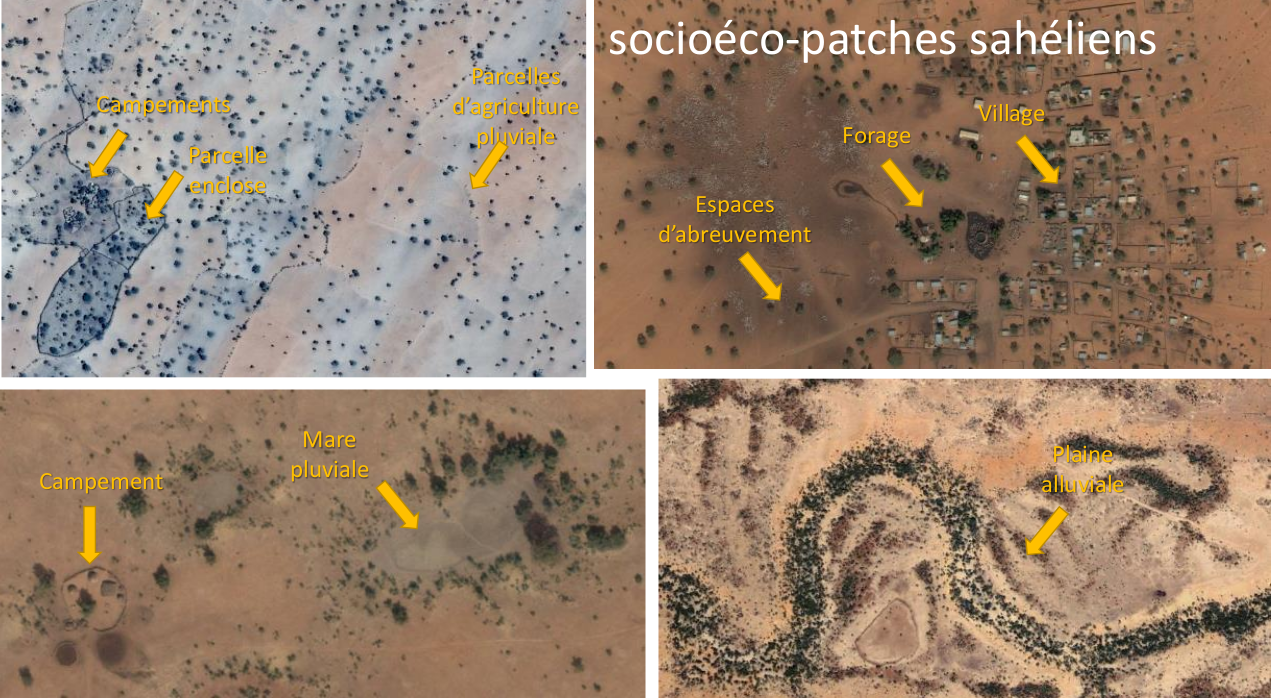
\includegraphics[width = 12cm]{img/patches.png}
\end{figure}

\end{frame}

\begin{frame}[c]{L'approche écologie du paysage 3/4}
\vspace{-1cm}

\begin{figure}
  \hspace*{-0.5cm}
	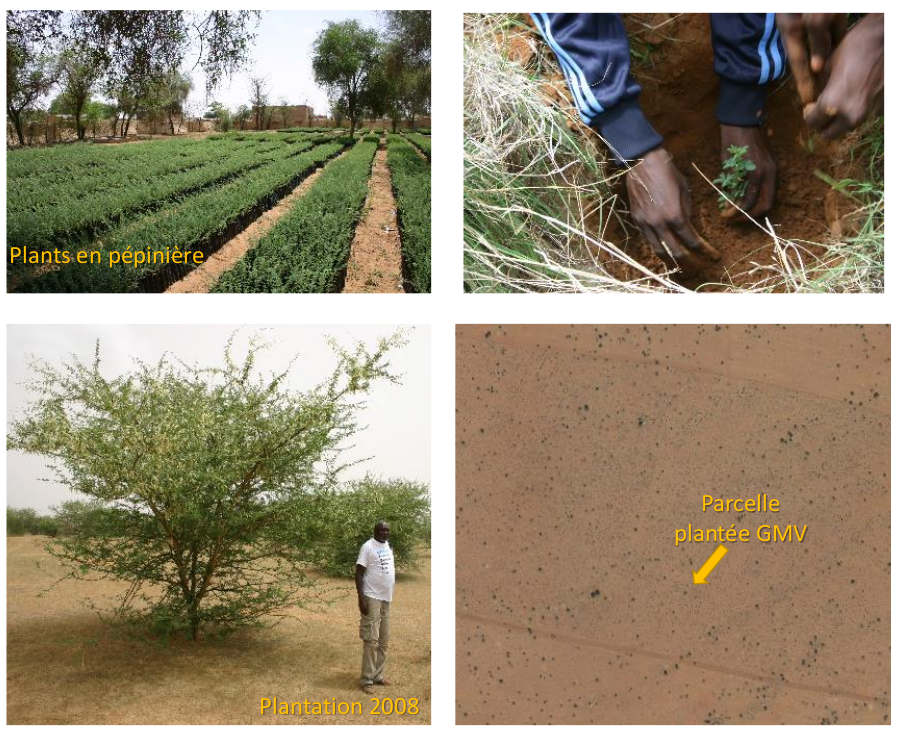
\includegraphics[width = 9cm]{img/patches2.png}
\end{figure}

\end{frame}


%-=-=-=-=-=-=-=-=-=-=-=-=-=-=-=-=-=-=-=-=-=-=-=-=
%	FRAME: Ecologie du paysage
%-=-=-=-=-=-=-=-=-=-=-=-=-=-=-=-=-=-=-=-=-=-=-=-=
\begin{frame}[c]{L'approche écologie du paysage 4/4}
\vspace{-1cm}
\begin{figure}
  \hspace*{-0.80cm}
	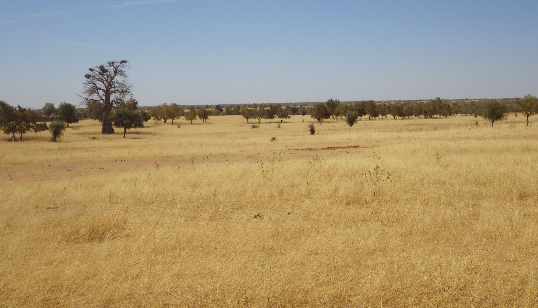
\includegraphics[height = 3.5cm]{img/pasto1.jpg}
  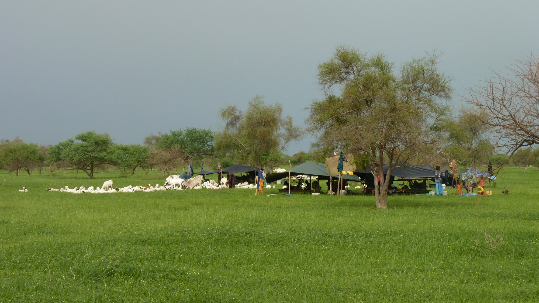
\includegraphics[height = 3.5cm]{img/pasto2.jpg}
  \caption{Zone pastorale}
\end{figure}

\end{frame}

%-=-=-=-=-=-=-=-=-=-=-=-=-=-=-=-=-=-=-=-=-=-=-=-=
%	FRAME: Participation
%-=-=-=-=-=-=-=-=-=-=-=-=-=-=-=-=-=-=-=-=-=-=-=-=
\section{methodologie - la demarche participative}
\begin{frame}[c]{Les ateliers}
\vspace{-1cm}
Un travail en ateliers avec pour objectif de faire évaluer par les acteurs l'importance des arbres dans chaque structure du paysage.
\begin{figure}
	\centering
	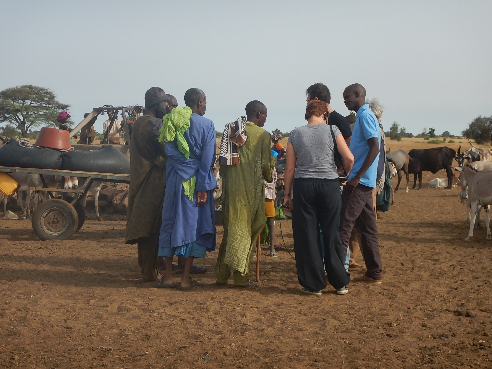
\includegraphics[width = 0.6\textwidth]{img/group1.png}
\end{figure}
\end{frame}


%-=-=-=-=-=-=-=-=-=-=-=-=-=-=-=-=-=-=-=-=-=-=-=-=
%	FRAME: Intégration à ComMod
%-=-=-=-=-=-=-=-=-=-=-=-=-=-=-=-=-=-=-=-=-=-=-=-=
\begin{frame}[c]{De l'arbre à la démarche ComMod}
\vspace{-1cm}
Une approche interdisciplinaire :
\begin{itemize}
  \item le travail d'enquête ethnobotanique permet d'identifier des pratiques socio spatiales
  \item coupler au travail d'écologie du paysage, on identifie spatialement la contribution des lieux aux pratiques des habitants
  \item La formalisation des pratiques et de l'identification des lieux conduit à la formalisation de modèles de comportement et donc à une approche prospective validée par les acteurs.
\end{itemize}
\end{frame}

%-=-=-=-=-=-=-=-=-=-=-=-=-=-=-=-=-=-=-=-=-=-=-=-=
%	FRAME: ANR framework in 4 wp
%-=-=-=-=-=-=-=-=-=-=-=-=-=-=-=-=-=-=-=-=-=-=-=-=
\begin{frame}[c]{La démarche ComMod}
\vspace{-1cm}
Un premier travail à été fait sur la base d'un modèle déjà documenter (Railsback et Grimm, 2011) : "Mushroom Hunting".

%%% Movie
\begin{center}
    \movie[width=4cm,height=4cm,poster]{}{video/hunter.webm}
\end{center}

On peut explorer l'importance de différents paramètres (distance, visibilité, mémoire, etc.) sur des réplications à grande échelle (analyse de sensibilité).
\end{frame}

%-=-=-=-=-=-=-=-=-=-=-=-=-=-=-=-=-=-=-=-=-=-=-=-=
%	FRAME: ANR framework in 4 wp
%-=-=-=-=-=-=-=-=-=-=-=-=-=-=-=-=-=-=-=-=-=-=-=-=
\begin{frame}[c]{Une complexification}
\vspace{-1cm}
Vers un modèle spatialement réaliste (pose la question de la réalité).

\begin{figure}
	\centering
	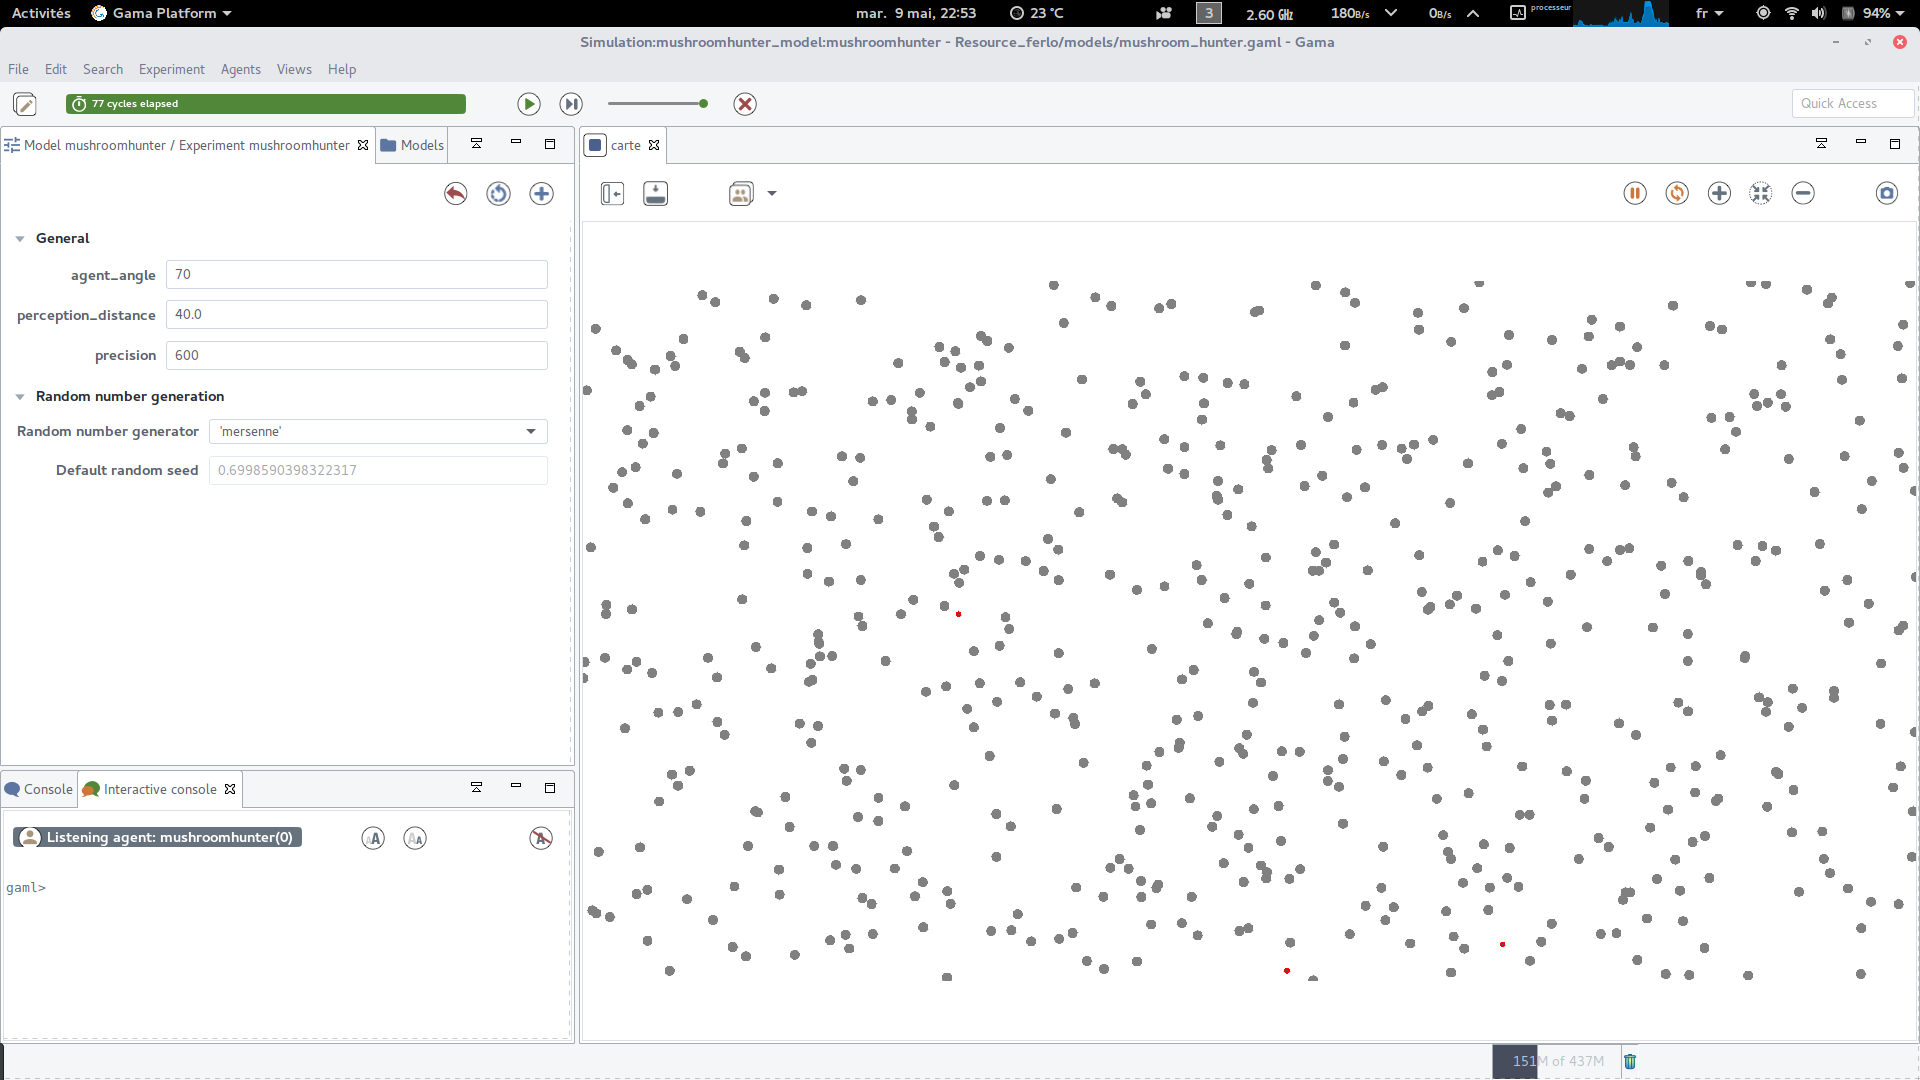
\includegraphics[width = 0.8\textwidth]{img/gama_ferlo}
	\caption{Proto model avec GAMA 1.7}
\end{figure}
\end{frame}


%-=-=-=-=-=-=-=-=-=-=-=-=-=-=-=-=-=-=-=-=-=-=-=-=
%	FRAME: Discussion
%-=-=-=-=-=-=-=-=-=-=-=-=-=-=-=-=-=-=-=-=-=-=-=-=

\section{Resultats attendus}


%-=-=-=-=-=-=-=-=-=-=-=-=-=-=-=-=-=-=-=-=-=-=-=-=
%	FRAME: Conclusion
%-=-=-=-=-=-=-=-=-=-=-=-=-=-=-=-=-=-=-=-=-=-=-=-=

\begin{frame}[c]{Résultats attendus}
\vspace{-1cm}
\begin{itemize}
  \item analyser les pratiques des populations sur les ressources provenant de la végétation arborée,
  \item identifier la manière dont ces populations perçoivent les changements dans leur environnement et les répercussions que cela a sur leurs pratiques,
  \item projeter dans le temps ces changements de pratiques pour évaluer leurs impacts sur les socio-écosystèmes sahéliens.
\end{itemize}
\end{frame}


%-=-=-=-=-=-=-=-=-=-=-=-=-=-=-=-=-=-=-=-=-=-=-=-=
%	FRAME: MERCI DE VOTRE ATTENTION
%-=-=-=-=-=-=-=-=-=-=-=-=-=-=-=-=-=-=-=-=-=-=-=-=
{
\usebackgroundtemplate{
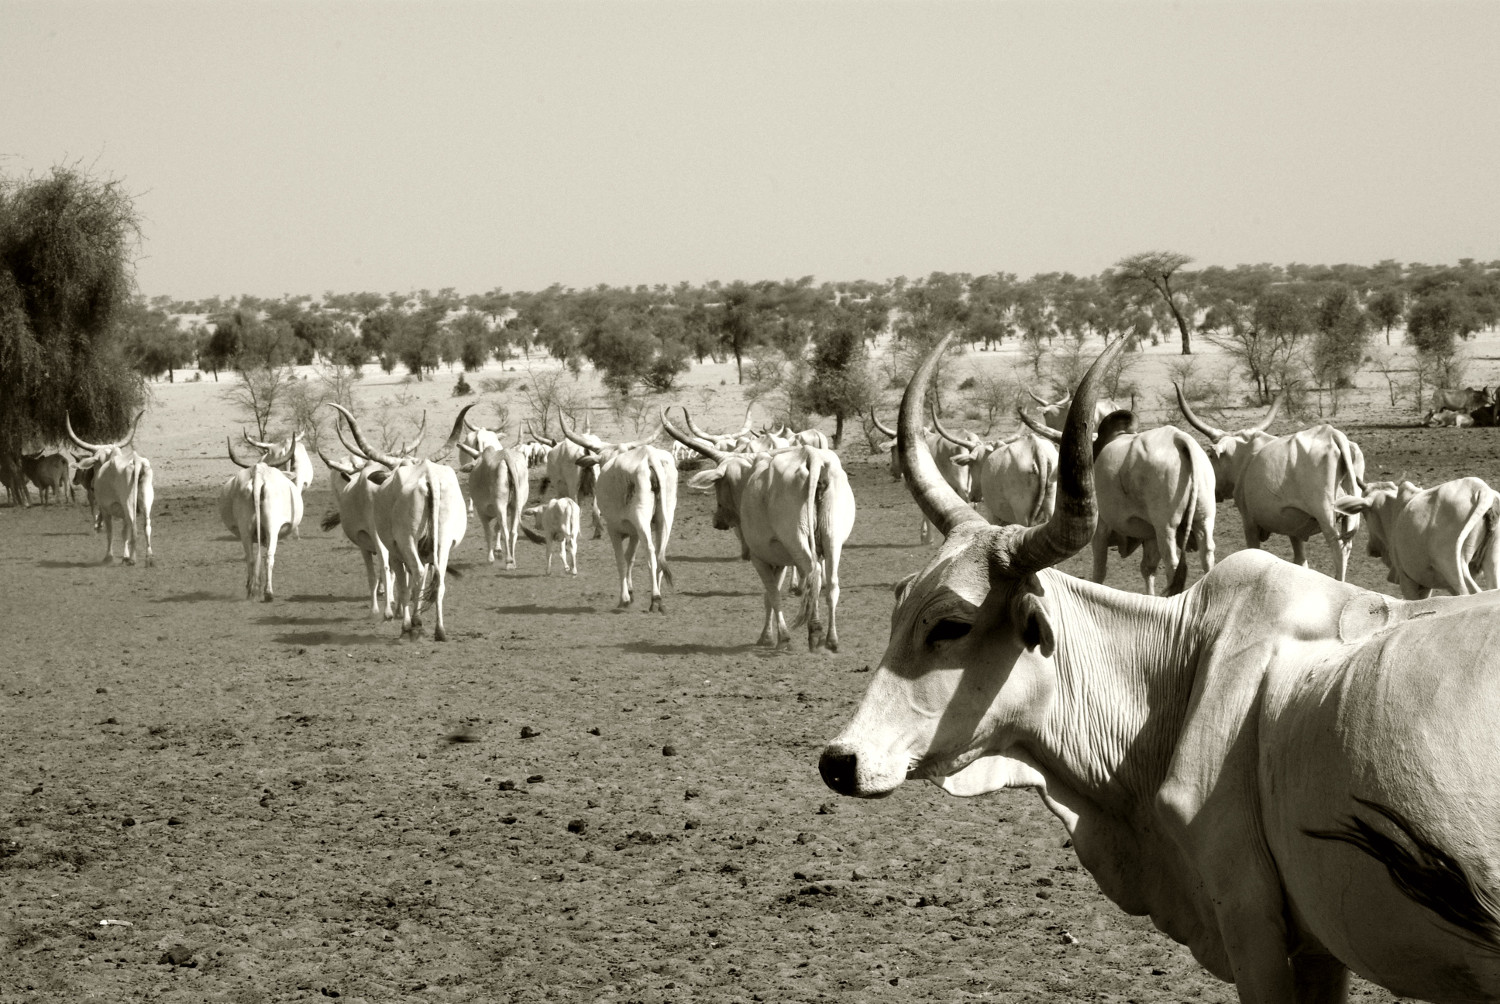
\includegraphics[width=\paperwidth]{img/podor_fin}}%
\begin{frame}
  \vspace{-1em}
  \begin{minipage}[t][.8\textheight]{\textwidth}
    \color{\cnGrey}{\LARGE{Thank you for your attention}}

    \vfill

  %\hfill \small{Photo credit : Thomas m-louis. sur \includegraphics[height=0.55cm]{img/flickr_logo}}
  \end{minipage}
  \vspace{-3.5em}
  \centering
	You can find this presentation on github
\includegraphics[height=0.85cm]{img/github}

\end{frame}
}


\end{document}
